\documentclass[times, utf8, diplomski, english]{fer}
\usepackage{booktabs}
\usepackage{footnote}
\usepackage{graphicx}
\usepackage{mathtools}
\usepackage{pdfpages}

\usepackage{listings}
\usepackage{protobuf/lang}  % include language definition for protobuf
\usepackage{protobuf/style} % include custom style for proto declarations.
\usepackage[hidelinks]{hyperref}

\DeclareMathOperator*{\argmin}{\arg\!\min}
\DeclareMathOperator*{\argmax}{\arg\!\max}
\graphicspath{{./figures/}{./fig_gen/}}

\begin{document}

\thesisnumber{1572}
\title{ End-to-End Deep Learning Model for Base Calling of MinION Nanopore Reads}
\author{Neven Miculinić}
\maketitle
 

\includepdf[pages={1,2}]{zadatak.pdf}

\zahvala{I would like to thank my mentor, Mile Šikić, for his patient guidance, encouragement
    and advice provided over the years.
    
I would also like to thank my family and friends for their
    continuous support.
    
In the end, honorable mentions go to Marko Ratković for his help with this thesis.    
}

\tableofcontents
\listoffigures

%%%%%%%%%%%%%%%%%%%%%%%%%%%%%%%%%%%%%%%%%
% Chapter Introduction
%%%%%%%%%%%%%%%%%%%%%%%%%%%%%%%%%%%%%%%%%
\chapter{Introduction}
\label{chap:Introduction}
In recent years, deep learning methods significantly improved the state-of-the-art in multiple domains such as computer vision, speech recognition, and natural language processing~\citep{LeCun:1998:CNI:303568.303704, NIPS2012_4824}
In this paper, we present application of deep learning for DNA basecalling problem.

Oxford Nanopore Technology's MinION nanopore sequencing platform~\cite{mikheyev2014first} is the first portable DNA sequencing device. It produces longer reads than competing technologies. In addition, it enables real-time data analysis which makes it suitable for various applications.
Although MinION is able to produce long reads, even up to 882 kb~\cite{loman1-100k,loman2-800k}, they have an error rate of 10\% or higher. This master thesis uses R9.4 pore model and compares previous techniques with novel auto-encoder multi-task training. 

\section{Organization}
Chapter~\ref{chap:background} covers the sequencing technologies basics, Oxford Nanopore Technologies(ONT) sequencing model, and available solutions to MinION sequencing. 
Chapter~\ref{chap:methods} covers common concepts, most from deep learning, used throughout this thesis. 
Chapter~\ref{chap:system_arhitecture} covers the whole system architecture and important programming system parts. 
Chapter~\ref{chap:results} goes into result analysis from the experiments.
Chapter~\ref{chap:discoure} reflects on the overall problem and voices author's opinion on related topics.
Finally, in chapter~\ref{chap:conslusion} this thesis final words are uttered in the closing statement. 

%%%%%%%%%%%%%%%%%%%%%%%%%%%%%%%%%%%%%%%%%
% Chapter Background
%%%%%%%%%%%%%%%%%%%%%%%%%%%%%%%%%%%%%%%%%

\chapter{Background}
\label{chap:background}
Due to technical constraints, it's infeasible to sequence whole DNA in a single strand. 
Every sequencing technology to date has an upper limit how big strand can it precisely sequence.
This limit is considerably smaller than the size of the genome.
For example, E.Coli has ~4.5 million base pairs in its DNA, while Sanger's sequencing maximum output is around 1000 base pairs max.
To make DNA basecalling feasible technique called shotgun sequencing was invented. 
The strand is cloned number of times, then via chemical agent broken down into smaller fragments of appropriate length. 
Sequenced fragments are called reads.

Genome assembly is the process of reconstructing the original genome from reads and usually starts with finding overlaps between reads.
The quality of reconstruction heavily depends on the length and the quality (accuracy) of the reads produced by the sequencer. 

If we have reference sequence we usually align the reads on the reference to aid us in the genome assembly. Otherwise, we have to use de novo assembly techniques.

The right analogy would be building a puzzle. Since we cannot scan the whole puzzle because our camera is too small or imprecise, we are scanning pieces of the whole picture. Puzzle pieces would represent fragments in this analogy. If we have a map, even a rough one, it shall aid us in assembling those puzzle pieces into complete pictures. Otherwise, we're fiddling in the dark and using de novo assembly techniques.

Figure \ref{fg:sequencing} depicts process of sequencing visually.

\begin{figure}[!ht]
    \begin{center}
        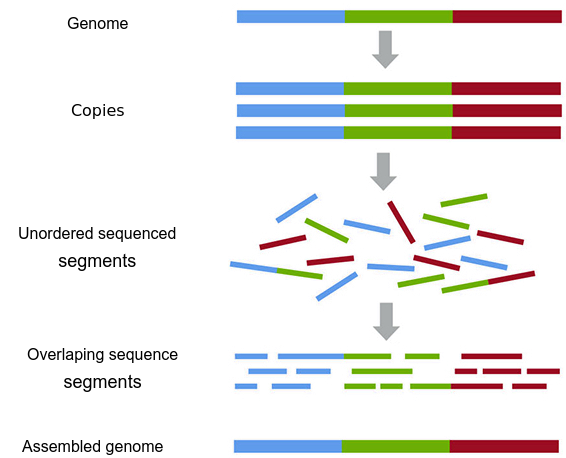
\includegraphics[width=0.6\textwidth]{shotgun-sequencing}
        \caption{Depiction of the sequencing process}
        \label{fg:sequencing}
    \end{center}
\end{figure}


In 1977, Frederick Sanger~\citep{mile}\citep{Pettersson2009} started development of sequencing technologies. It allowed reading lengths up to 1000 bases with very high accuracy(99.9\%) at the cost of 1\$ per 1000 bases.
Later, seconds generation sequencing, like IAN Torrent and Illumina devices, reduced the price while keeping the accuracy high. However, they had a cost of shorter read lengths, about a few hundred base pairs, which makes resolving repetitive regions practically impossible.

Repeated regions are patterns of nucleic acids (base pairs) that occur in multiple copies throughout the genome. 

Third generation sequencing technologies have longer read lengths at the accuracy's expense. PacBio, for example, developed technology with a few thousand bases with error rates of \textasciitilde10-15\%. 

MinION sequences, which this master thesis use, made sequencing more portable.

\section{Oxford Nanopore MinION}

The MinION device by Oxford Nanopore Technologies is the first portable DNA sequencing device. Its small weight, low cost, and long read length combined with decent accuracy yield promising results in various applications including full human genome assembly \cite{human_seq} what could potentially lead to precision medicine. It weighs only 87 grams, and its portability leads to uses on the international space station and the Antarctic among other places.

Under the hood, it has numerous nano-meter sized pores, thus a names Nanopore. Each pore has a depth of around 6 nucleotides. Under electric current DNA strand passing through the pore and changes its electric resistance. The sensor measures the current through the pore multiple times a second~\footnote{The model we worked with had 4000 samples per seconds}. This signal varies depending which k-mer is occupying the pore, and on its basis, we're performing the basecalling. On figure~\ref{fg:nanopore} this process is visually depicted. 

MinION devices can produce long reads, usually tens of thousand base pairs (with reported reads lengths of 100 000\cite{loman1-100k} and even recently above 800 000 base pairs \cite{loman2-800k}), but with higher sequencing error than older generations of sequencing technologies.

\begin{figure}[!ht]
    \begin{center}
        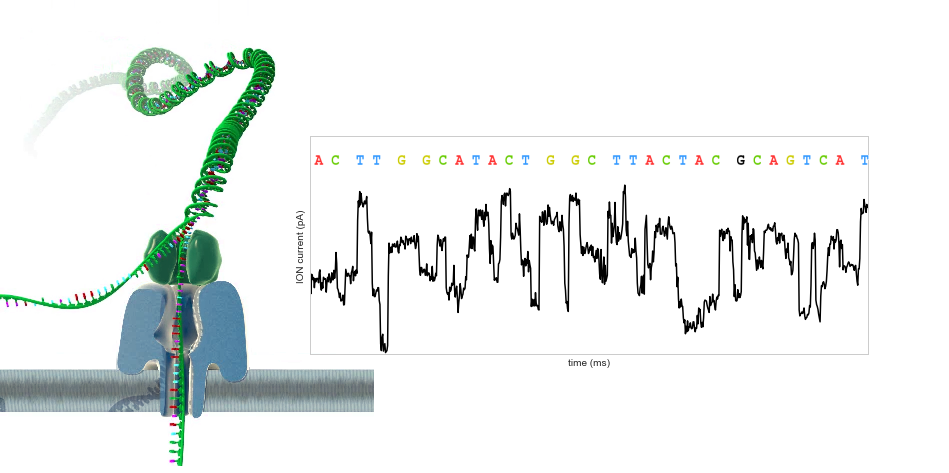
\includegraphics[width=0.8\textwidth]{nanopore}
        
        \caption[DNA strain being pulled through a nanopore]{DNA strain being pulled through a nanopore \protect\footnotemark}
        \label{fg:nanopore}
    \end{center}
\end{figure}
\footnotetext{Figure adapted from https://nanoporetech.com/how-it-works}

The sequencing resulting file is in FAST5 format, which is adapted HDF5 file format, popular in the bioinformatics community. It stores raw signal, alongside various metadata. Unfortunately, many basecallers, including the official ones, upon executing store their results in the FAST5 files. It leads to data and processing coupling in single file and bloated file sizes. 

\begin{figure}
    \begin{center}
        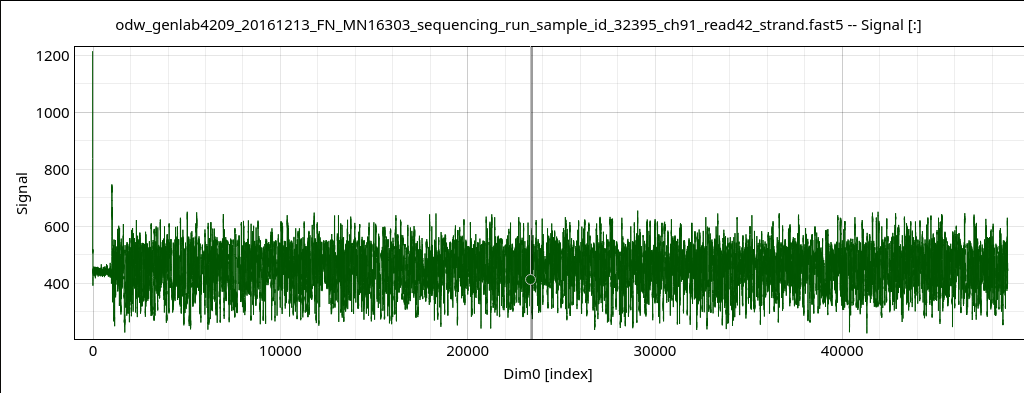
\includegraphics[width=\textwidth]{fast5_sample}
        \caption[Structure of FAST5 file and raw signal plot show in \textit{HDFView}]{Structure of FAST5 file and raw signal line plot show in \textit{HDFView} \protect\footnotemark}
        \label{fg:fast5}
    \end{center}
\end{figure}
\footnotetext{https://support.hdfgroup.org/products/java/hdfview/}
  
\section{Related work}

\subsection{Oxford Nanopore Technologies}
This subsection covers various basecallers published by ONT, the MinION device maker.
\subsubsection{Metrichor}

Metrichor is a defunct cloud-based basecaller. The older versions used \textit{hidden Markov models} (HMM) as the underlying algorithm. Preprocessing started with segmenting signal into smaller chunks called events with their start, end, length, mean signal strength and standard deviation. These events are observations in the HMM model, and the underlying generating hidden sequence is the sequence of 6-mers. They build their HMM transition matrix with stay, skip 1 and skip 2 probabilities, that is underlying 6-mer cannot move for more than 2 nucleotides per event. Basecalling is performed using the Viterbi algorithm. This approach showed poor results when calling long homopolymer stretches as the context in the pore remains the same \cite{homopolymers}\cite{homopolimeri_analiza}.

\subsubsection{Nanonet}
Nanonet is ONT first-generation neural network basecaller. It used to be available on GitHub, but it's now defunct and unavailable.

\subsubsection{Albacore}
Albacore is a production basecaller provided by Oxford Nanopore Technologies and uses a command-line interface. It
utilizes the latest in Recurrent Neural Network algorithms in order to interpret the signal data from the
nanopore and basecall the DNA or RNA passing through the pore. It implements stable features into
Oxford Nanopore Technologies’ software products, and is fully supported. It receives .fast5 files as an
input, and is capable of producing: 
\begin{itemize}
    \item .fast5 files appended with basecalled information
    \item .fast5 files that have been processed, but basecall information present in a separate .fastq file
\end{itemize}

\subsubsection{Guppy}
Guppy is ONT's new basecaller that can use GPUs to basecall much faster than Albacore. Both the GridION X5 and PromethION contain GPUs and use Guppy to basecall while sequencing. Guppy can also use CPUs and scales well to many-CPU systems, so it may run faster than Albacore even without GPUs.  In the future, it's intended to replace Albacore as production basecaller.
\subsubsection{Scrappie}
Scrappie\footnote{\url{https://github.com/nanoporetech/scrappie}} is ONT's research basecaller. Scrappie is reported to be the first basecaller that specifically address homopolymer base calling. It became publicly available just recently in June 2017 and supports R9.4 and future R9.5 data.

Unlike Albacore, Scrappie does not have fastq output, either directly or by writing it into the fast5 files – it only produces fasta reads.

\subsection{Third-party basecallers}

\subsubsection{Nanocall}
Nanocall~\citep{David046086} was the first third-party open source basecaller for nanopore data. It uses HMM approach like the original R7 Metrichor. Nanocall does not support newer chemistries after R7.3.

\subsubsection{DeepNano}
DeepNano~\citep{Boza2017}  was the first open-source basecaller based on neural networks. It uses bidirectional recurrent neural networks implemented in Python, using the Theano library. When released, originally only supported R7 chemistry, but support for R9 and R9.4 was added recently.
\subsubsection{basecRAWller}
basecRAWller~\footnote{\url{https://basecrawller.lbl.gov/}} is developed by Marcus Stoiber and James Brown at the Lawrence Berkeley National Laboratory.

\subsubsection{Chiron}
Chiron~\citep{chiron_teng} is developed by Haotian Teng and others in Lachlan Coin's group at the University of Queensland. They are basecalling from the raw signal, first using a residual convolutional neural network, than LSTM and finally beam search or greedy decoder depending on chosen configuration. 

\chapter{Methods}
\label{chap:methods}
This chapter is dedicated to explaining key deep learning concepts used throughout the master thesis. It's here primarily for completeness, and it's author recommendation to go into detail via other sources, for example, Deep learning book~\citep{deep_learning_book-Goodfellow-et-al-2016}, google, or research papers cited for most of the techniques. TensorFlow~\citep{tensorflow2015-whitepaper} and Keras~\citep{chollet2015keras} deep learning frameworks were used for implementation. For some deep learning concept, I'll provide equivalent keras/tensorflow code whichever one is simpler and used throughout the codebase. 

\section{Neural Network}
The feed-forward Neural network is the basic building block of any deep learning system. It's composition of multiple differentiable functions. Commonly we have input vector $x$, apply some linear transformation to it and add bias, and finally on the result some activation function. Details on common choices for activation function are in section~\ref{sec:activation}. In mathematical language $y = f(Ax + b)$ would be one layer of neural network transforming input $x$ into output $y$. Stacking those operations we get multiple layers, hence the word deep in deep learning. Simple 3-layer neural network is depicted in figure~\ref{fg:nn}.

\begin{figure}[!ht]
    \begin{center}
        \begin{align*}
            y_1 &= f(A_1x + b_1) \\
            y_2 &= f(A_2y_1 + b_2) \\
            y &= f(A_3y_2 + b_3) \\
        \end{align*}
        \caption{Simple three layer feed forward neural network}
        \label{fg:nn}
    \end{center}
\end{figure}

\section{Activation functions}
\label{sec:activation}

Most neural network operations are a linear transformation. Composing multiple linear transformations we get the new linear transformation. Thus have non-linear behavior we use the non-linear activation functions. Originally, the most popular choice was $\tanh$ and $\sigma(x) = \frac{1}{1 + e^{-x}} $ activation functions. They are nice because of limited output domain. 

However, other choices proved more effective, especially with deep neural network due to greater learning speeds, and to overcome gradient vanishing problem. Gradient vanishing refers to neural network gradient approaching zero as we backpropagate through more and more layers. Exploding gradient is related phenomena in which gradient approaches infinity. Both present serious hampering to neural network training.

ReLU, The rectified linear unit, $f(x) = \max(0, x)$,  is one hugely popular choice and decent baseline compared to other ReLU variants. ReLU greatly accelerates the convergence of stochastic gradient descent compared to $\sigma$ and $\tanh$ activation functions~\citep{NIPS2012_4824}. 

Furthermore, its calculation is drastically simpler than computing transcendental functions, like $\sigma$ or $\tanh$.

Over time, ReLU showed its downsides, called \textit{dying ReLU}. It still saturates the gradients when it's 0, that is when $x <= 0$ giving no useful gradient to back propagate. Thus several ReLU variant have been proposed: PrRelu~\citep{prelu} in equation~\ref{eq:prelu}, ELU~\citep{elu} in equation~\ref{eq:elu}, and finally SeLU~\citep{selu} in equation~\ref{eq:selu}. In Selu constants $\alpha$ and $\lambda$ are chosen in such a way that output gravitates towards normal distribution with zero mean and unit variance. Those constants are: $\lambda = 1.0507$ and $\alpha = 1.6732$. 
Code generating the function plot is displayed in figure~\ref{fg:actcode}, and the plot is in figure~\ref{fg:act_plot}

\begin{equation}    
\label{eq:prelu}
PrELU(x)=
\begin{cases}
x & \text{if}\ x>0 \\
\alpha x & \text{otherwise}
\end{cases}\\
\end{equation}

\begin{equation}
\label{eq:elu}
ELU(x)=
\begin{cases}
x & \text{if}\ x>0 \\
\exp(x) - 1 & \text{otherwise}
\end{cases}    \\
\end{equation}

\begin{equation}
\label{eq:selu}
\text{selu}(x)= \lambda
\begin{cases}
x & \text{if}\ x>0 \\
\alpha e^x - \alpha & \text{otherwise}
\end{cases} 
\end{equation}

\begin{figure}
\begin{lstlisting}[language=python,style=protobuf]
import tensorflow as tf
import keras
import seaborn as sns
import numpy as np
import matplotlib.pyplot as plt

for act in ["relu","selu", "elu"]:
    with tf.Graph().as_default():
        x = tf.placeholder(shape=(None, ), dtype=tf.float32)
        y = keras.layers.Activation(act)(x) 

        with tf.Session() as sess:
            xx = np.linspace(-1, 1)
            yy = sess.run(y, feed_dict={
                x: xx
            })
            plt.plot(xx, yy, label=act)
            plt.legend()
\end{lstlisting}
\caption{Code generating the activation function plot. Also shows how tensorflow and keras could be used}
\label{fg:actcode}
\end{figure}

\begin{figure}
    \begin{center}
        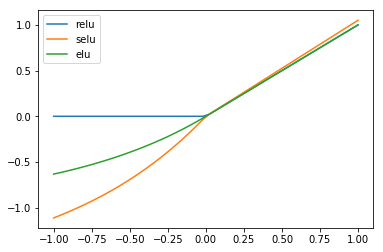
\includegraphics[width=0.8\textwidth]{act_plot}
        \caption{Plot of common activation functions between -1 and 1. PrELU is excluded since the parameter $\alpha$ is learnt during training}
        \label{fg:act_plot}
    \end{center}
\end{figure}

\section{CNN}
Convolutional Neural Networks(CNN) are the bread and butter of almost all computer vision system today, and they launched the deep learning hype with unprecedented results on Image Classification problems. 
Lately, their scope is expanded to Natural language processing (NLP) tasks with promising results~\citep{BYTENET, facebook}.

Convolution is a type of feed-forward neural network layer where the weights are tied together. We have a sliding window over which we apply a linear transformation of the input, and get the output element. This operation is repeated to get the full output tensor. For 1D case~\footnote{\url{https://keras.io/layers/convolutional}} figure~\ref{fg:convolution} depicts it visually. 

There's also atrous convolution~\cite{atrous_DBLP:journals/corr/ChenPSA17}, also known as dilated convolution where spaced input tensor elemets are taken depending on the dilation factor. Ordinary convolution is a special case with $\text{dilation} = 1$.

\begin{figure}
    \begin{center}
        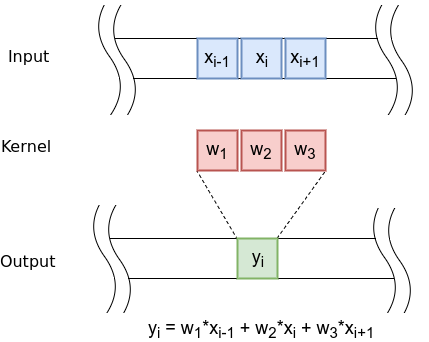
\includegraphics[width=0.5\textwidth]{convolution}
        \caption{Convolution layer, kernel size 3 with stride 1. Adapted from~\citep{mratkovic} with authors permission.}
        \label{fg:convolution}
    \end{center}
\end{figure}

\section{RNN}
RNN, residual neural networks are one of the basic building blocks in sequence models. They are feed-forward neural network spanned in a time domain. The same neural network is applied to two inputs, hidden state and input at time $t$ and gives two outputs, new hidden state, and output at time $t$. The historic information remains saved in the hidden state, and it's propagated to the future. Its visual description is depicted in figure~\ref{fg:rnn}.

\begin{figure}[!ht]
    \begin{center}
        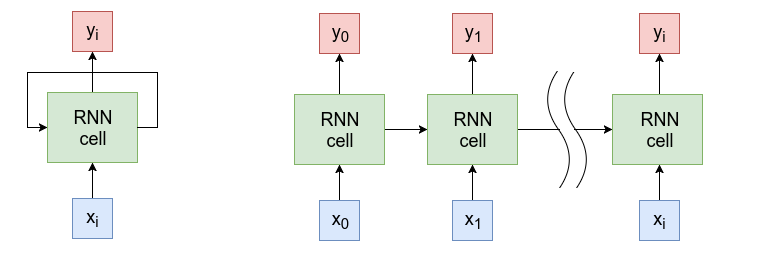
\includegraphics[width=0.8\textwidth]{rnn}
        \caption{An unrolled recurrent neural network. Adapted from~\citep{mratkovic} with authors permission.}
        \label{fg:rnn}
    \end{center}
\end{figure}


They can be unrolled in one massive feed-forward neural network. They are trained with backpropagation through time, on this unrolled graph. Usually the unrolling is capped and fixed number or time steps. 
A common issue to vanilla RNNs is vanishing and exploding gradients problem. It's solved by redesigning the basic RNN cell. There are two common approaches called LSTM~\citep{hochreiter1997long} and GRU~\citep{gru}.

Bidirectional Recurrent Neural (BiRNN) networks are used when the current output not only depends on the previous elements in the sequence but also future elements. Basically, we're stacking to RNNs, one in a forward direction and another in the backward and concatenating the hidden states/outputs. This approach was used in DeepNano~\citep{Boza2017}.

Despite their modeling power, the main drawback is their speed. Since they are processing data sequentially, it's hard to parallelize those operations. 

\section{Pooling layer}
Pooling layers refer to tensor dimensionality reduction. Tensor is squeezed by some factor, and each block of factor width is aggregated using some aggregation function. 
In other words, we divide our tensor into equally shaped hyperrectangles, and each aggregate using aggregation function yielding new hyperrectangle. 
Fox example, maxPool2d for image sized 50x50 shall with pool size (2,2) divides it into rectangles of size (2, 2) max those 4 elements and result in image sized 25x25.
This is visually depicted in figure~\ref{fg:maxpool}.
Common choices are AvgPool, and MaxPool~\citep{Scherer:2010:EPO:1886436.1886447}~\footnote{\url{https://keras.io/layers/pooling/}}.

\begin{figure}
    \begin{center}
        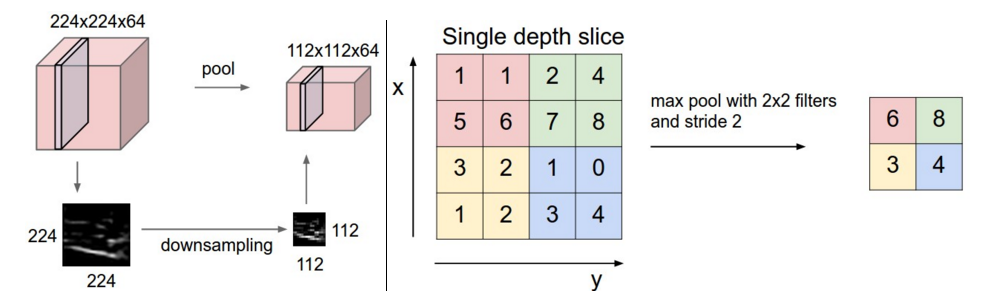
\includegraphics[width=0.8\textwidth]{Pooling_Simple_max}
        \caption{Example of max pool layer in convolutional neural network. Adapted from~\url{https://leonardoaraujosantos.gitbooks.io/artificial-inteligence/content/pooling_layer.html}}
        \label{fg:maxpool}
    \end{center}
\end{figure}

\section{CTC loss}
\label{sec:ctc_loss}

How do you measure how much are two sequences similar in the differentiable manner? If we were using classing encoder/decoder architecture with RNN's there's only one way to output the target sequence, and we'd optimize our RNN's outputs logits to match the target 1-hot encoded vector. 

However, in this architecture, we're outputting logits whose size depend only on the input signal size. First, let's start with some alphabet, $\Sigma = \{A, G, T, C\}$ of the output symbols we're using.  
Let's say the target sequence is \texttt{AAG} and we're having 5 logits due to input signal constraints. 
Logits have shape $[\text{sequence length}, \text{num classes}]$. 
What is the ideal logit values to get this target sequence to the output? 
First, we must define how the sequence is decoded. 
The logit sequence is decoded by finding the most likely path through the logits at each time step $t$. Our logits can be represented as on figure~\ref{fg:ctc_graph_0}.
But we're presented with a problem, if we pick path \texttt{AAAAG} how do we finally decode this sequence as target \texttt{AAG}? The solution proposed in original paper for Connectionist Temporal Classification(CTC)~\citep{Graves:2006:CTC:1143844.1143891, ctc-blog} is indeed brilliant. 
We introduce a special blank symbol, $-$. Whenever model outputs blank symbol it's taken as nothing more than padding and class separator. 
That way our logits can output \texttt{A-A-G} which shall decode in the target sequence.
But what about \texttt{AA--G}? How is this decoded when there are consecutive repeated classes in the most probable path. 
Decoding depends on which CTC variant we used during training. There's option to \texttt{merge\_repeated}, that is decode \texttt{AAA-G} as \texttt{AG}, or if it's false decode it as \texttt{AAAG} by simply dropping the blanks. 

\begin{figure}
    \begin{center}
        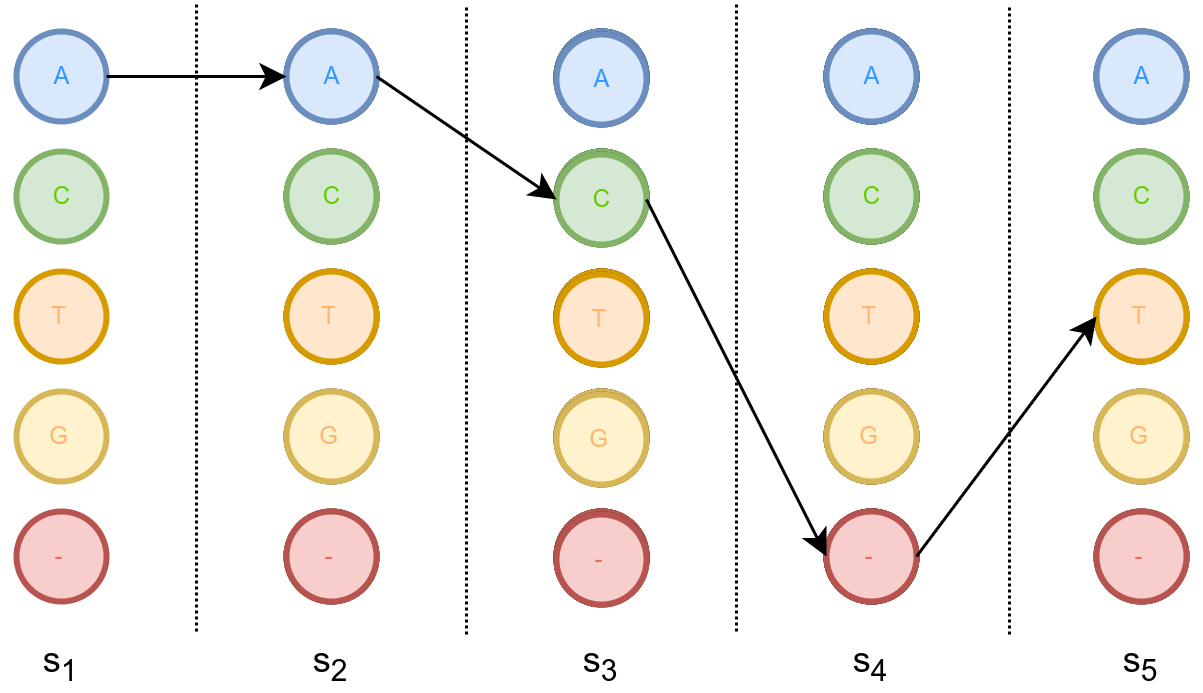
\includegraphics[width=0.8\textwidth]{ctc_graph_1}
        \caption{Depiction of CTC decoding. At each time step we're picking one class, and the probability of this path is the product of probabilities at each time step for that class. Equivalently, in log domain it's the sum of log probabilities, that is logits. Adapted from~\citep{mratkovic}}
        \label{fg:ctc_graph_0}
    \end{center}
\end{figure}

Now, let's get back to the original problem. What's the probability our sequence is \texttt{AAG} under those logits. 
The solution is summing probabilities for all paths which decode into target sequence. 
Or in mathematical language, we define function decoded as out decoding procedure. 
Path probability is the product of probabilities per time step in the path, as in equation~\ref{eq:ctc_path_prob}.
An example can be seen in equation~\ref{eq:multiple}. 
Then the probability of our text being equal \texttt{AAG} is given by equation~\ref{eq:ctc_prob}.
This is a procedure we can optimize with usual MLE~\footnote{maximum likelihood estimator}, the common loss in machine learning area.

\begin{equation}
\begin{gathered}
\label{eq:ctc_path_prob}
P(\pi | X) = \prod_{t=1}^{m} o_t(\pi_t), \\
\text{where $o_t(\pi_t)$ is probability of element $\pi_t$ being $t^{th}$ element on path $\pi$}
\end{gathered}
\end{equation}

\begin{equation}
\begin{gathered}
\label{eq:multiple}
AAG = \begin{cases}
decode(A, -, A, -, G) \\
decode(A, A, - -, G) \\
\vdots \\
decode(A, -, -, A, G) 
\end{cases}
\end{gathered}
\end{equation}

\begin{equation}
\begin{gathered}
\label{eq:ctc_prob}
P(y = \text{AAG}| \text{logits}) = \sum_{\pi \in decode^{-1}(\text{AAG})} P(\pi | \text{logits})
\end{gathered}
\end{equation}

\subsection{Beam search decoding}
\label{subsec:beam-search}

All is fine and dandy during training, but during inference, we're left with a computationally intensive problem. Enumerating all paths lead to exponential complexity, things we'd like to avoid. Even smart dynamic programming solutions shall use more resources then feasible for any non-trivial length sequence. 

To battle this problem we have 2 solutions. First is using greedy approach, and find the path such that we're picking the most probably class at each time step, and composing path out of it.

Better approximation, however, is between those two extremes, greedy and exhaustive search. Beam search decoding~\cite{graves_decode}. At each time step, we're only looking at top $N$ paths up until this point. Parameter $N$ is called beam width. From time $t$ to $t+1$ we have dynamic programming transitions, where we look at all possible path continuations and keep only the best $N$ ones until reached the end. Then we output the best one as our decoded path, apply post-processing (merge repeated if configure in that mode, drop blanks) and we're done.

\section{Autoencoder}
\label{sec:autoencoder}
Autoencoders are a type of neural network where the output target is the input target~\footnote{Unless we're talking about denoising autoencoder for which the input has additional noise}. They funnel the data through smaller and smaller layers until we're reaching the neural network bottleneck -- a thought vector as Geoffrey Hinton calls it.  From there multiple layers are stacked on top of each other until we get the input back. In it's basic for they're quite simple, input $x$, output $y$ and loss some loss function which measures the similarity between $x$ and $y$. Variations include denoising autoencoder~\citep{vincent2008extracting}, variational autoencoder (VAE)~\citep{kingma2013auto}, U-net~\citep{DBLP:journals/corr/RonnebergerFB15} and many others. 

\section{Multi task training}
Multi-task learning~\footnote{\url{http://ruder.io/multi-task/}}~\citep{multi-task-learning,Caruana1997,DBLP:journals/corr/abs-1106-0245} is approach where we're optimizing multiple tasks on the same dataset. 
It has been shown it may lead to better performance than learning a specific model for each task. 
So far it has been successfully applied in many domains, including natural language processing~\citep{Collobert:2008:UAN:1390156.1390177}, speech recognition~\citep{speech_multitask}, computer vision~\citep{cv-multitask}, drug discovery~\citep{ramsundar2015massively} and many other areas. 

In the context of MinION basecalling, I combine two tasks. 
The first one is basecalling the sequence, that is deriving appropriate logits which shall minimize CTC loss defined in section~\ref{sec:ctc_loss}, and autoencoder reconstruction original signal from said logits using \texttt{L2} loss for distance measurement~\footnote{Maybe it would be better using dynamic time warping distance measurement, however, due to technical requirements of implementing in tensorflow the author chose the simpler option. This would be future work section} between signals. 

The idea is this additional loss helps models learn better logits by training on not only one but two tasks. In chapter~\ref{chap:results} you can see the detailed analysis of this approach.


%%  ######  ##    ##  ######  ######## ######## ##     ##    ###    ########  ##     ## #### ######## ########  ######  ######## ##     ## ########  ######## 
%% ##    ##  ##  ##  ##    ##    ##    ##       ###   ###   ## ##   ##     ## ##     ##  ##     ##    ##       ##    ##    ##    ##     ## ##     ## ##       
%% ##         ####   ##          ##    ##       #### ####  ##   ##  ##     ## ##     ##  ##     ##    ##       ##          ##    ##     ## ##     ## ##       
%%  ######     ##     ######     ##    ######   ## ### ## ##     ## ########  #########  ##     ##    ######   ##          ##    ##     ## ########  ######   
%%       ##    ##          ##    ##    ##       ##     ## ######### ##   ##   ##     ##  ##     ##    ##       ##          ##    ##     ## ##   ##   ##       
%% ##    ##    ##    ##    ##    ##    ##       ##     ## ##     ## ##    ##  ##     ##  ##     ##    ##       ##    ##    ##    ##     ## ##    ##  ##       
%%  ######     ##     ######     ##    ######## ##     ## ##     ## ##     ## ##     ## ####    ##    ########  ######     ##     #######  ##     ## ######## 

\chapter{System architecture}
\label{chap:system_arhitecture}
\section{Data Preparation}
\label{sec:data_preparation}
In previous project implementation, we used fast5 with additional custom .ref files as our dataset. This setup had some issues. First, it was IO heavy since we were reading the whole fast5 file which contained non-raw data section~\footnote{like basecalling from other basecallers}, data management with separated raw files and labels, and lastly it was a magic to parse it every time. Which exactly group or subgroup within fast5, or is the signal start normalized to 0, or is it some arbitrary begging written at some other place in fast5 files changes from version to version. 

Therefore, for this project, I've decided to make my own custom format for training described via protobuf~\citep{protobuf}. The issue from previous versions wasn't the only reason. Another was ease of importing other peoples data in their formats into this one. If I can read it, I can easily write plugin converting between formats. As of writing this thesis, 4 such plugins were written since I wasn't sure which data I shall use and in which format am I going to import them in. 

Ease of machine encoding/decoding as well as other previously mentioned factors guided this decision. Also, I've written datapoint format inspector operating on this common format, making my life easier. The source code for conversion procedures can be found on minion-data~\footnote{\url{https://github.com/nmiculinic/minion-data}} GitHub repository as well as pypi. The specific interface description language(IDL) can be seen in figure~\ref{fg:dataset_proto}.


\begin{figure}
    \begin{center}
    \begin{lstlisting}[language=protobuf3,style=protobuf]
syntax = "proto3";

package dataset;

enum BasePair {
    A = 0;
    C = 1;
    G = 2;
    T = 3;
    BLANK = 4;
}

enum Cigar {
    MATCH = 0;
    MISMATCH = 1;
    INSERTION = 2; // Insertion, soft clip, hard clip
    DELETION = 3;  // Deletion, N, P
}

message DataPoint {
    message BPConfidenceInterval {
        uint64 lower = 1;
        uint64 upper = 2;
        BasePair pair = 3;
    }
    repeated float signal = 1;
    repeated BasePair basecalled = 2; // What we basecalled
    repeated BPConfidenceInterval labels = 3; // labels describe corrected basecalled signal for training
}
    \end{lstlisting}
    \caption{dataset protobuf description}
    \label{fg:dataset_proto}
    \end{center}
\end{figure}

\subsection{Data correction}
Each data point has been previously basecalled, and some resulting sequence was obtained. Then each sequence was corrected by aligning to the reference genome. By aligning to the reference we get the reference genome region and the CIGAR strings describing the alignment. The CIGAR string is list ordered sequence of insertions(I), deletions(D), matches(=) and mismatches(X). Insertions are bases present in the query string but absent from reference, and deletions are the opposite. 

Example alignment is depicted in figure~\ref{fg:align}. We take the error corrected labels and place them in dataset protobuf file for further training processing.

\begin{figure}
    \begin{center}
        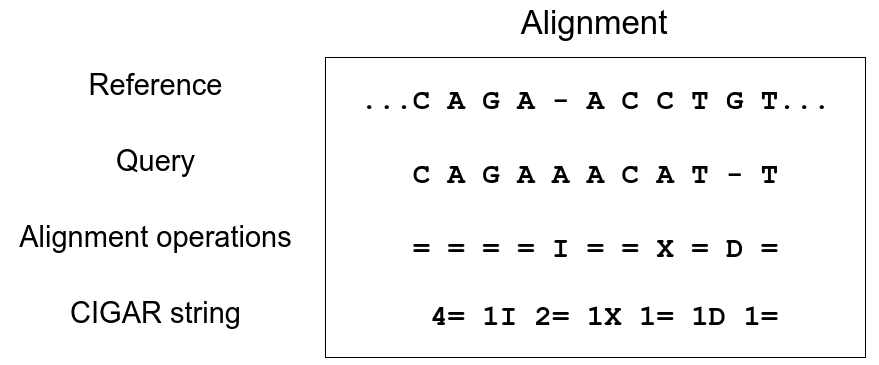
\includegraphics[width=0.6\textwidth]{alignment}
        \caption{Example of simple alignment and CIGAR string. Adapted from~\citep{mratkovic}}
        \label{fg:align}
    \end{center}
\end{figure} 

\subsection{Data sources}

Raw data has been acquired from Jared Simpson's E.Coli sequenced with R9.4 pore chemistry. 

It's been basecalled by Metrichor and corrected after aligning to reference using graphmap. 
It consists of 90 thousands read divided into train set (60k) and validation set (30k)
The devision is performed depending on read position on reference genome. 
This way, further statistical bias is avoided if read's are sampled from the same genome region.

% Data has been downloaded from \url{https://data.genomicsresearch.org/Projects/online_dataset/train_set_all/}.  The following species were provided there by the Chiron team:
% \begin{itemize}
    %\item Human
    %\item E. Coli
    %\item Lambda Phage
%\end{itemize}

% For the concrete Chiron dataset, the re-squiggled preparation method was used. (The data was re-squiggled, that is after aligning the read on the reference, the read data is improved and each base pairs place on the raw signal is calculated.)
% The re-squiggled basecalled data is located at \verb|/Analyses/RawGenomeCorrected_000/BaseCalled_template/Events|. The interesting code fragments are in function processDataPoint of file \verb|minion_data/preperation/_re_squggled.py| from minion-data python package.
% After the gzipped dataset is prepared, it goes into the training pipeline. The whole training \& testing pipeline is available  open source on \url{https://github.com/nmiculinic/minion-basecaller}

\section{Training pipeline}
After getting data in the uniform format, the training part comes next. In aiming this as observable and simple as possible I've modeled config in using python3 \texttt{typing.NameTuple}~\footnote{\url{https://docs.python.org/3/library/typing.html}} and voluptuous for data validation. 
With those two tools, I've created statically typed configuration file format and data validation with a human-readable error. As serialization format, I've chosen YAML for its readability and terseness. 
The config file definiton is in figure~\ref{fg:train_cfg_py} and example config file for training is in figure~\ref{fg:train_cfg_yml}. The source code can be found in module \texttt{mincall.train.\_train.py} and we're recommending reading it for extended details.

\begin{figure}
    \begin{center}
    \begin{lstlisting}[language=python,style=protobuf]
class TrainConfig(NamedTuple):
    model_name: str
    train_data: List[DataDir]
    test_data: List[DataDir]
    logdir: str
    seq_length: int
    batch_size: int
    surrogate_base_pair: bool

    train_steps: int
    init_learning_rate: float
    lr_decay_steps: int
    lr_decay_rate: float

    model_hparams: dict = {}
    grad_clipping: float = 10.0
    validate_every: int = 50
    run_trace_every: int = 5000
    save_every: int = 2000

    tensorboard_debug: str = ""  # Empty string is use CLI debug
    debug: bool = False
    trace: bool = False

    @classmethod
    def schema(cls, data):
        return named_tuple_helper(
            cls, {
                'train_data': [DataDir.schema],
                'test_data': [DataDir.schema],
            }, data
        )

    \end{lstlisting}
    \caption{dataset protobuf description}
    \label{fg:train_cfg_py}
    \end{center}
\end{figure}

\begin{figure}
    \begin{center}
    \begin{lstlisting}[]
version: "v0.1"
train:
  train_data:
    - name: "r9.4"
      dir: "./mincall/example"
  test_data:
    - name: "r9.4"
      dir: "./mincall/example_test"
  model_name: "dummy"
  model_hparams:
    num_layers: 5
  surrogate_base_pair: false
  train_steps: 60
  init_learning_rate: !!float 1e-4
  lr_decay_steps: 10000
  lr_decay_rate: 0.5
  seq_length: 40
  batch_size: 10
  logdir: "./logs"
    \end{lstlisting}
    \caption{training config yaml}
    \label{fg:train_cfg_yml}
    \end{center}
\end{figure}

Input data is read via background thread which processes it, packages it into signal and label slices, and pushed into tensorflow space queues. Inside those queues, data is shuffled, and composed into batches for further training. This part of the code has an extensive test suite, including end2end tests with the golden file~\footnote{golden file is test technique where you save function output to the golden file, verify manually it's correct, and after each successive test, you're checking that nothing changed. This way we can be sure refactoring didn't influence correctness.}

From configuration rest of the pipeline is initialized. This included model, with its hyperparameters, loading config defined train and test sets, learning rate schedule, sequence lengths, batch size and other settings. Keras is used for model definition due to its simplicity in design. 

Additionally, I've embedded edlib~\citep{edlib} in the tensorflow's \texttt{tf.py\_func} operation which enabled me having match, mismatch, insertion, deletion and identity rates observer during training on both train and test set.

Standard python logging module was used with multiple backends. One backend saved to log file for further inspection. The other one shipped logs to graylog system which I've set up on faculty servers. This system enabled me to log searching and greater efficiency in finding bugs. 

Example command for starting the training procedure is shown in figure~\ref{fg:train_cfg_sh}.

\begin{figure}
    \begin{center}
    \begin{lstlisting}[language=bash,style=protobuf]
docker run --rm -it -u="$(id -u):$(id -g)" \
-v $DATA_DIR:/data:ro  \
-v $MODEL_DIR:/model \ 
nmiculinic/mincall:latest-py-gpu train --config /model/config.yml
    \end{lstlisting}
    \caption{Example of starting training command. In the config model is properly configures to use \texttt{/data} and \texttt{/model} paths}
    \label{fg:train_cfg_sh}
    \end{center}
\end{figure}

\section{Hyperparameter optimization}

Our models have various hyperparameters. For example, learning rate, receptive width size, number of blocks, etc. To gain a better model we're not only optimizing models parameters, but also hyperparameters on the validation set. For this, I've implemented hyperparam search capabilities in the programming solution. 

The design rationally does as little things as possible. It takes the training configuration with injected hyperparams, and it creates a new directory and \texttt{config.yml} for each new hyperparam assignment. Then it releases control to the training code part as if we had run training on the command as previously described in figure~\ref{fg:train_cfg_sh} making this maximally observable. After the training completes it reports back to the hyperparam controller the results and according to backing hyperparameter optimization procedure new assignment is calculated.

There are two concrete hyper-optimization strategies implemented. One is random search, and other is sigopt~\footnote{\url{https://sigopt.com}}. 
I've primarily used sigopt as the main hyper-optimization strategy.

Its config is similar to the training and its NamedTuple definition can be seen in figure~\ref{fg:hyper_cfg_py}. The param is flexible entry; it can be a single scalar value, and then it's not hyper-optimized, or it can be a dictionary with \texttt{type} field and other fields depending on the parameter types, e.g. int, float, categorical, etc. 

\begin{figure}
    \begin{center}
    \begin{lstlisting}[language=python,style=protobuf]
class HyperParamCfg(NamedTuple):
    model_name: str
    train_data: List[DataDir]
    test_data: List[DataDir]
    seq_length: Param
    batch_size: Param
    surrogate_base_pair: Param

    train_steps: Param
    init_learning_rate: Param
    lr_decay_steps: Param
    lr_decay_rate: Param

    model_hparams: Dict[str, Param]

    work_dir: str
    grad_clipping: float = 10.0
    validate_every: int = 50
    run_trace_every: int = 5000
    save_every: int = 2000
    \end{lstlisting}
    \caption{HyperParameter options description}
    \label{fg:hyper_cfg_py}
    \end{center}
\end{figure}

\subsection{Basecalling}
\label{subsec:basecalling}

Basecalling is performed using either beam search decoder explained in subsection~\ref{subsec:beam-search} or greedy search 
decoding~\footnote{It's similar to beam search with beam width 1, that is we greedily take the most likely symbol at each time step}.

However, it's often infeasible passing whole signal through the GPU and the model. 
Then we divide the signal into overlapping stripes, calculate logits from each stipes and assembly the final read. 

There are two possible strategies. We can combine the stripes in the logits space, and perform beam search/greedy search on them, 
or we first perform beam search/greedy search on them and combine the stripes in the reading space. 

I've opted out for the former option. 
Combining them in logits space is a pretty simple pattern -- by overlaying stripes in reversed order.
There's one caveat here, combining in logit space works best when the model is history independent, e.g.
using only CNN layers without RNN layers which have hidden state. I have a hunch it should work alright with RNN's too but I haven't tested it.

A Picture is worth a thousand words, and this process is depicted in figure~\ref{fg:logit_comp}

\begin{figure}
\begin{center}
\begin{verbatim}
1111111122223333
11111111........
....22222222....
........33333333
\end{verbatim}
\end{center}
\caption{Process of overlapping stripes in logit space. Number signal from which stripe the logit information comes and at the top composite logit is assembled.}
\label{fg:logit_comp}
\end{figure}

An alternative approach is used in Chiron~\citep{chiron_teng} where they first decode each stripe, then assemble them. 
The assembly process works by overlapping consecutive stripes, thus getting relative offset, then using consensus on each output position.
This approach requires a greater deal of overlap between stripes, unlike in logit space, which leads to slower basecalling.
They also use RNN's, which naturally have a performance length limit. 
Their sequence length is around 300, and relative signal offset around 30, 
while in mincall sequence lengths are around 100k with offsets around 90k. Actually for mincall, sequence lenght is limited only by GPU memory since logit inference process is easily parallelizable due to extensive CNN usage. 

\subsection{Final model arhitecture}
\label{subsec:final-model-architecture}

The final model has residual layer architecture, with Gated residual layer residual blocks~\citep{resnet,DBLP:journals/corr/Savarese16}. 
It's composed of stacked blocker intertwined with max-pooling layers.
Each block is composed of multiple residual layers. 
Whole composition is visually depicted in figure~\ref{fg:final_arch}.
For the best mode, \texttt{num\_blocks} is 2 and \texttt{num\_layers} is 9.
In the backward pass, in an autoencoder stage, we take the logits and use the same architecture with maxPools replaced with Upsampling1D layers.
Combined loss is calculated as $\text{total loss} = \text{autoenc\_coeff} * \text{autoencoder L2 loss} + \text{ctc loss}$.
During the hyperparemeter serach the best possible \texttt{autoenc\_coeff} is 32.875. 

\begin{figure}
    \begin{center}
        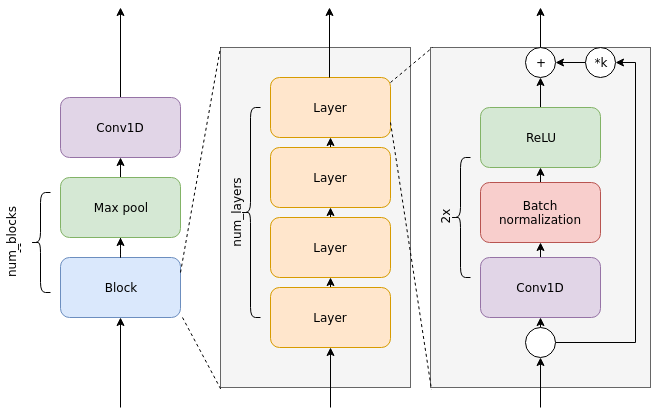
\includegraphics[width=0.8\textwidth]{final_arch}
        \caption{Final arhitecture overview}
        \label{fg:final_arch}
    \end{center}
\end{figure}

\chapter{Results}
\label{chap:results}

\section{Definitions}
We're measure two things. Each read is aligned to the reference genome and multiple metrics are measured, defined at the end of this section in figure~\ref{fg:metrics}. However, the reads don't tell the whole picture since we're interested in the final product, consensus assembly of reads. The reads could have a systemic bias in the same regions and suffer from same errors which would yield subpar consensus versus reads correcting each other and yielding better consensus accuracy than any read on their own.

The consensus is generated from pileup using a simple algorithm. We simply align all the reads to the genome, stack them on top of each other forming pileup of read bases. Bases are called using majority vote. Deletions are handled if there's majority call for deletion, and for insertion, there has to be majority length and the bases of insertion. 

In figure~\ref{fg:consensus} shows how consensus is called from pileup created from aligned reads. 

\begin{figure}
    \begin{center}
        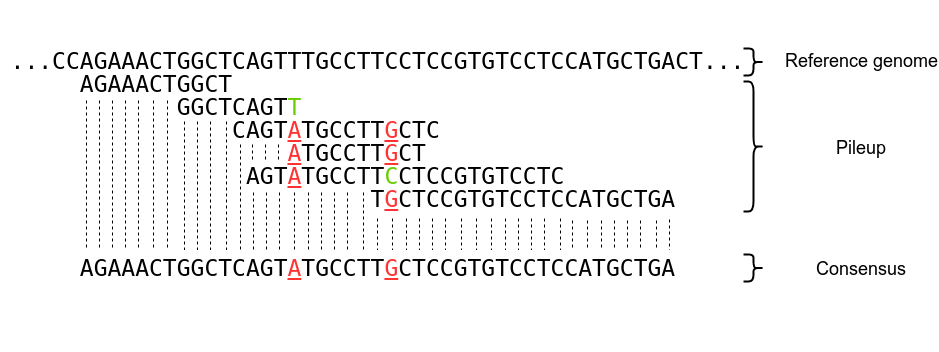
\includegraphics[width=0.8\textwidth]{consnesus}
        \caption{Consensus from pileup. Adapted from~\citep{mratkovic}}
        \label{fg:consensus}
    \end{center}
\end{figure}

After both consensus and read, alignment is calculated, we can represent the sequence alignment with CIGAR string, that is a sequence of matches(=), mismatches(X), insertions(I) and deletions(D). Additionally, at the beginning and end of the read alignment, soft(S) and hard(H) clips may be present which are removed. Additionally, padding information(P) and spliced alignment skip cigar(N) is likewise stipped from the analysis. These conventions are taken from SAM file format definitions. In the end, we're left with the following metrics as defined in figure~\ref{fg:metrics}.

\begin{figure}
\begin{align*}
 \text{read\_length} &= \#(=) + \#(X) + \#(I) \\ 
 \text{match\_rate} &= \frac{\#(=)}{\text{read\_length}} \\
 \text{mismatch\_rate} &= \frac{\#(X)}{\text{read\_length}} \\
 \text{insertion\_rate} &= \frac{\#(I)}{\text{read\_length}} \\
 \text{deletion\_rate} &= \frac{\#(D)}{\text{read\_length}} \\
 \text{identity\_rate} &= \frac{\#(=)}{\#(=) + \#(X) +\#(I) + \#(D)}  
\end{align*}
\caption{Various perfomance measurement metrics as defined throughout this thesis.}
\label{fg:metrics}
\end{figure}

On his GitHub repo, Ryan Wick composed multiple basecaller comparasion~\citep{rwick_basecalling_cmp}~\footnote{\url{https://github.com/rrwick/Basecalling-comparison}}. 
This section briefly summarizes his work and it's recommended to check original authors work, it's quite good! 
Due to resource constraints both time and compute, I'm unable to run my own testing on my data with each basecaller. Thus I'm reusing Ryan's Wick's basecalled files for my analysis. 

\section{Mincall}
All previously mentioned metrics are displayed here. In figure~\ref{fg:identity_rate} is this solution compared to other basecallers on dataset proposed by~\citep{rwick_basecalling_cmp}.
Figure~\ref{fg:tbp:all_metrics} provides mean per read statistics for all previously defined metrics. 
For mincall, I've also calculated a distribution of each CIGAR operation (I, D, X, and =) over the relative reads length in figure~\ref{fg:error_distribution}.
Figure~\ref{fg:concensus_report} reports various consensus related metrics once all reads are assembled together.
Finally, I compare basecalling speeds between greedy search and beam search with the beam width of 50 in figure~\ref{fg:basecaller_speed}. 
Here it's clearly visible how much of bottleneck beam search is.

\begin{figure}
    \begin{center}
        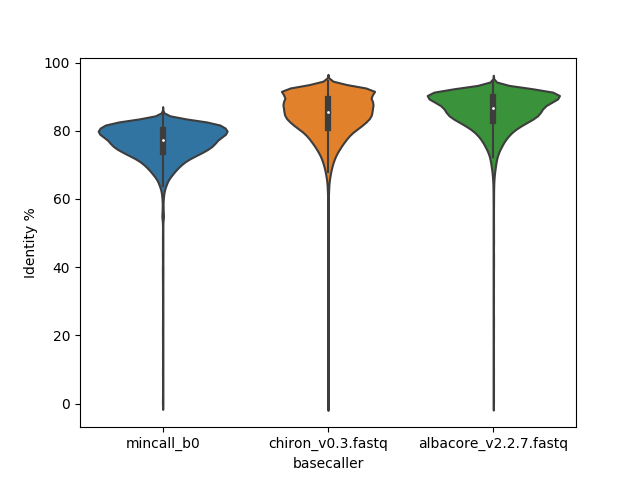
\includegraphics[width=\textwidth]{read_violin_Identity}
    \end{center}
    \caption{Basecallers read identity. All non-mincall ones are taken from~\cite{rwick_basecalling_cmp}}
    \label{fg:identity_rate}
\end{figure}

\begin{figure}
\begin{tabular}{lrrrrrrr}
\toprule
{} &    Error \% &    Match \% &  Mismatch \% &  Insertion \% &  Deletion \% &  Identity \% &  Read length \\
basecaller    &            &            &             &              &             &             &              \\
\midrule
alignment\_b0  &  32.585652 &  85.364048 &    9.794374 &     4.841578 &   17.949700 &   72.086729 &  4465.777778 \\
alignment\_b50 &  30.242361 &  85.607736 &    9.614377 &     4.777887 &   15.850097 &   73.422217 &  4556.555556 \\
\bottomrule
\end{tabular}

\caption{Mean read metrics across basecallers. All non-mincall ones are taken from~\cite{rwick_basecalling_cmp}}
\label{fg:tbp:all_metrics}
\end{figure}

\begin{figure}
    \begin{center}
        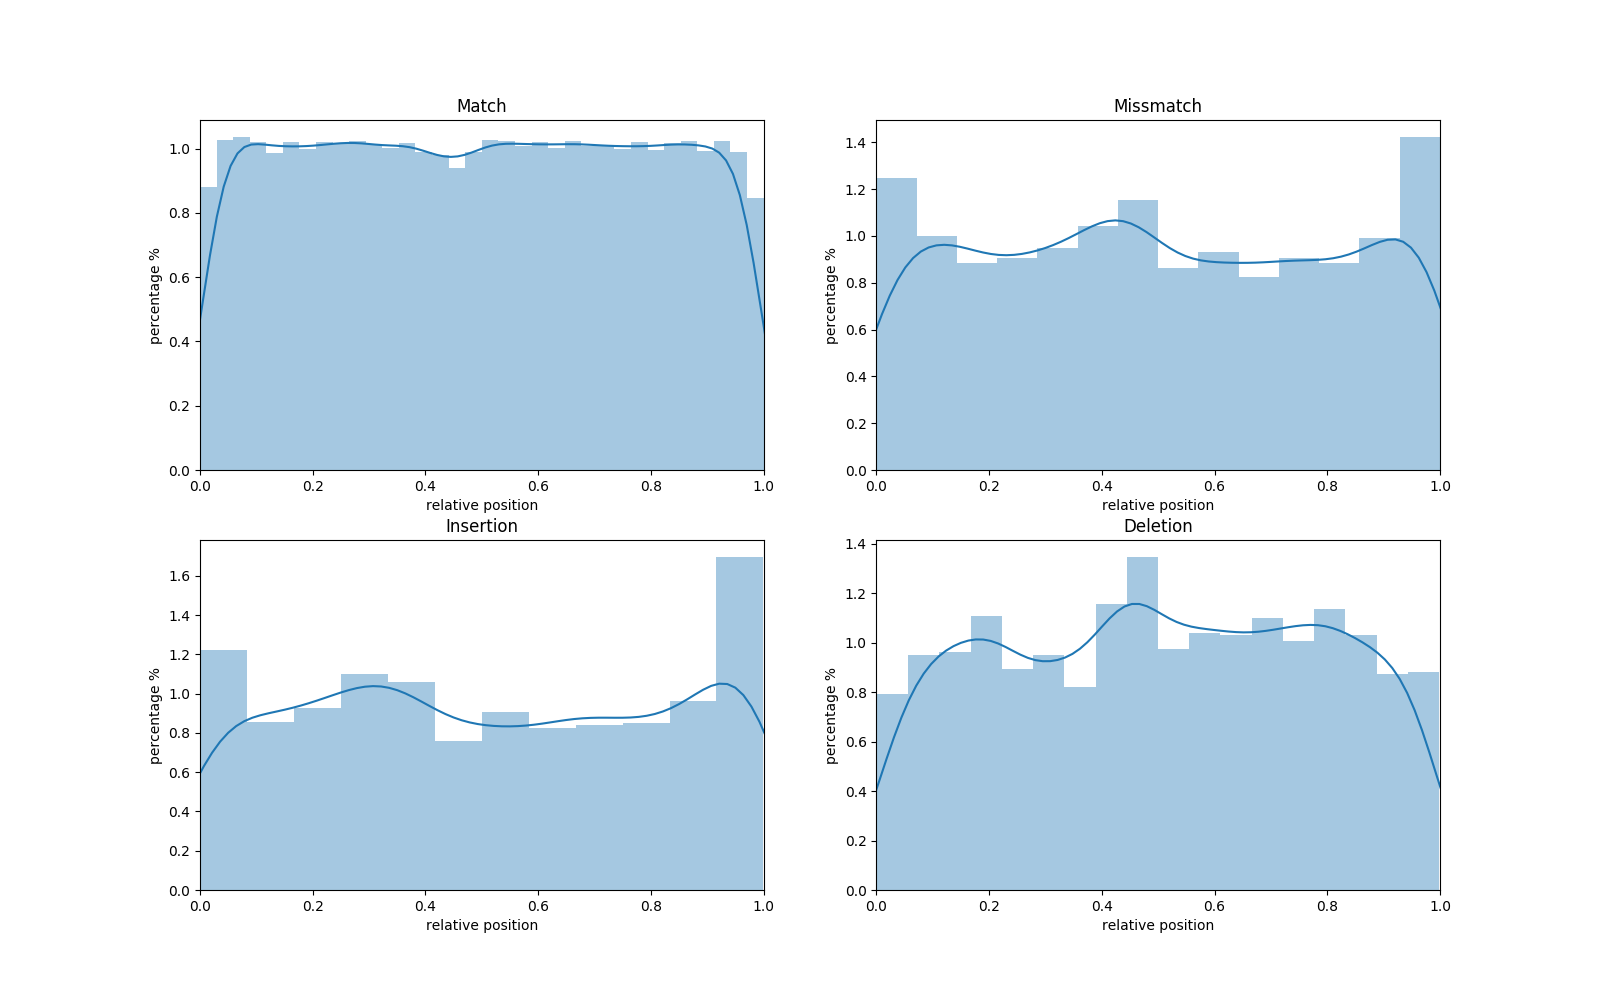
\includegraphics[width=\textwidth]{alignment_position_report.png}
    \end{center}
    \caption{CIGAR string distribution over the relative read position. Due to speed considerations performed only on small data subset.}
    \label{fg:error_distribution}
\end{figure}

\begin{figure}
\begin{tabular}{lrrr}
\toprule
{} &    mincall\_b0 &   mincall\_b50 &   chiron\_v0.3 \\
\midrule
coverage\_threshold     &           0 &            0 &            0  \\
snp\_count              &         754 &         1055 &          144  \\
insertion\_count        &          10 &           27 &            1  \\
deletion\_count         &         973 &         1049 &           84  \\
num\_undercovered\_bases &           0 &            0 &            0 \\
num\_called\_bases       &  5.5184e+06 &  5.51835e+06 &  5.51936e+06 \\
num\_correct\_bases      & 5.51763e+06 &  5.51727e+06 &  5.51921e+06 \\
average\_coverage       &     205.755 &      132.717 &      206.407  \\
snp\_rate               &   0.0136634 &     0.019118 &     0.002609  \\
insertion\_rate         & 0.000181212 &  0.000489277 &   1.8118e-05  \\
deletion\_rate          &   0.0176319 &    0.0190093 &   0.00152192  \\
correct\_rate           &     99.9862 &      99.9804 &      99.9974  \\
identity\_percentage    &     99.9671 &      99.9604 &      99.9957  \\
\midrule
{} &    albacore\_v2.2.7 &  guppy\_v0.5.1 & {} \\
\midrule
coverage\_threshold     &            0 &             0  & {} \\
snp\_count              &          296 &           296  & {} \\
insertion\_count        &           55 &            51  & {} \\
deletion\_count         &          214 &           202  & {} \\
num\_undercovered\_bases &            0 &             0 & {} \\
num\_called\_bases       &  5.51928e+06 &   5.51929e+06 & {} \\
num\_correct\_bases      &  5.51892e+06 &   5.51894e+06 & {} \\
average\_coverage       &      206.982 &       206.814  & {} \\
snp\_rate               &   0.00536302 &    0.00536301  & {} \\
insertion\_rate         &  0.000996508 &   0.000924032  & {} \\
deletion\_rate          &   0.00387732 &    0.00365989  & {} \\
correct\_rate           &      99.9936 &       99.9937  & {} \\
identity\_percentage    &      99.9904 &       99.9907  & {} \\
\bottomrule
\end{tabular}
\caption{Consensus report among the tested basecallers. All non-mincall ones are taken from~\cite{rwick_basecalling_cmp}}
\label{fg:concensus_report}
\end{figure}

\begin{figure}
\begin{tabular}{lrrr}
\toprule
{}                          &    Speed(bp/s) \\
decoding strategy           &                \\
\midrule
greedy search               &  178 412   \\
beam search (beam width 50) &  8 554     \\
\bottomrule
\end{tabular}
\caption{Basecaller speed depending on logit decoding strategy. All Tests were using Titan Xp GPU for logits and CPU for decoding on 32 core Intel Xeon E5-2640 @2Ghz}
\label{fg:basecaller_speed}
\end{figure}



\chapter{Discourse}
\label{chap:discoure}
During the development of the mincall, I've noticed a couple of things. 
First, as all the models are closely matched in their metrics, I suspect we've reached Bayesian error rate. 
Or we need the radically different approach to get further few \% improvements. 
Since the problem is quite simple without long-term dependencies, I'd guess Bayesian error rate is the more likely reason.

For further speed improvements, Beam Search implementation is the bottleneck. 
Usually, it's not used on long reads, and therefore it wasn't as optimized in tensorflow as it could have been since there was no need. 
While monitoring the basecalling process with \texttt{htop} utility I've noticed poor CPU utilization, that is for 10 parallel beam searches I'd expect 10 CPU's having 100\% utilization, but that wasn't the case indicating subpar performance.
This fate befalls all using beam search as their primary decoding mechanism, including Chiron~\citep{chiron_teng} and other projects. 
What Albacore uses underneath the hood isn't certain and I cannot comment on that. 

Most of the training is done on E. Coli, and lately, this set is expanded to the human genome and few other species. 
It would be beneficial gathering dataset in some standardized format with quality control. 
I've proposed the protobuf format and described it in section~\ref{sec:data_preparation}. 
Many other fields have their own Common Task Framework (CTF) benchmark, e.g. ImageNet, Cifar, etc. 
\chapter{Conclusion}
\label{chap:conslusion}

The goal of this thesis was explore new model in the MinION Basecaller space. 
I've opeted out using CNN on the raw waveform, and tried adding additional autoencoder loss to stabilize the trening. 
Judging by results, this autoencoded loss hasn't brought substantial benefit as I had hoped. 

In comparassion to state-of-the-art basecallers this solution is lagging behind, though it's my belief with refining it could be comparable.
For further precision improvements most likely candidate is the pore's perfomance and reducing pore's signal noise.

Additionally having two sensors in the pore, one measuring horizonatally and one vertically (that is across the pore) should provide greater accuracy and hopefully less error rates. This approach has been developing for quite some time, and we're yet to see the results. 

I'm hoping in the coming years this technology shall increase in speed, accuracy and affordability, leading to multiple novel application. 
As previously mentioned, knowing exact genome of our surroundings, e.g. infected wound, colon bacterias compositions or our own DNA variations enables
not only our deeper understanding, but also more efficient personalized medicine. 

We shall see what the future brings.

\bibliography{literatura}
\bibliographystyle{unsrtnat}
% \bibliographystyle{plainnat}

\begin{abstract}
In the MinION device, single-stranded DNA fragments move through nanopores, which causes drops in the electric current. The electric current is measured at each pore several thousand times per second. Each event is described by the mean and variance of the current and by event duration. This sequence of events is then translated into a DNA sequence by a base caller. Develop a base-caller for MinION nanopore sequencing platform using a deep learning architecture such as convolutional neural networks and recurrent neural networks. Instead of events, use current waveform at the input. Compare the accuracy with the state-of-the-art basecallers. For testing purposes use publicly, available datasets and Graphmap or Minimap 2 tools for aligning called reads on reference genomes.  Implement method using TensorFlow or similar library. The code should be documented and hosted on a publicly available Github repository.

\keywords{base calling, Oxford Nanopore Technologies, MinION, deep learning, seq2seq, convolutional neural network, residual network, CTC loss}
\end{abstract}

\hrtitle{S kraja na kraj model dubokog učenja za određivanje očitanih baza dobivenih uređajem za sekvenciranje MinION}
\begin{sazetak}
    Unutar uređaja MinION, fragmenti jednostruke DNA prolaze kroz nanopore, što uzrokuje promjene u električnoj struji. Struja proizvedena na svakoj nanopori mjeri se nekoliko tisuća puta u sekundi. Svaki događaj opisan je srednjom vrijednosti i varijancom struje te svojim trajanjem. Postupak kojim se takav slijed događaja prevodi u niz nukleotida naziva se određivanje očitanih baza. Razviti alat za prozivanje baza za uređaj za sekvenciranje MinION koristeći modele dubokog učenje kao što su konvolucijske i povratne neuronske mreže. Umjesto događaja na ulazu koristi valni oblik struje. Usporediti dobivenu točnost s postojećim rješenjima. U svrhu testiranja koristiti javno dostupne skupove podataka i alate GraphMap ili Minimap 2 za poravnanje očitanja na referentni genom. Alat implementirati koristeći programsku biblioteku TensorFlow (ili neku sličnu). Programski kod treba biti dokumentiran i javno dostupan preko repozitorija GitHub.
\kljucnerijeci{određivanje baza, Oxford Nanopore Technologies, MinION, duboko učenje, prevođenje, konvolucijske neuronske mreže, rezidualne mreže, CTC gubitak}
\end{sazetak}

\end{document}